% CONTRIBUTION: Q1 journal draft Rev.2 - supervisor correction 2026-10-08 (ported from THESIS Rev.2).
% Supervisor demands answered: (1) every section briefed What/Why/How + running example;
% (2) Where is agent? Sec 4.2 roster with file paths; (3) What is model? Sec 4.3 rules+frozen LLM, no training;
% (4) Orchestration architecture? Sec 4.4 contracts+sequence+timings+failures;
% (5) 120 refs + 60+ in-text cites; (6) related work 6 pillars + 15-rival gap matrix.
% Target: Expert Systems with Applications / Computers and Security. Paste into Overleaf, pdfLaTeX.
% Status: system + Eval-A 70 + Eval-Big 1995 complete; Eval-B human N=30 = protocol only (fill Sec 6.5 after run).
\documentclass[11pt,a4paper]{article}
\usepackage[margin=25mm]{geometry}
\usepackage{graphicx,amsmath,booktabs,hyperref,url,array,longtable}
\usepackage[utf8]{inputenc}
\hypersetup{colorlinks=true,linkcolor=blue,citecolor=blue,urlcolor=blue}
\title{FinLearn Guard: A Closed-Loop Agentic Platform Unifying Real-Time Cyber Threat Detection and Personalized Guided Response for Finance Staff}
\author{Poly Rani Ghosh\textsuperscript{1,*} \and Koushiq Chowdhury\textsuperscript{1} \\
\small \textsuperscript{1}Department of Computer Science and Engineering, Notre Dame University Bangladesh, Dhaka, Bangladesh \\
\small \textsuperscript{*}Corresponding author: polyghosh@ndub.edu.bd }
\date{\today}
\begin{document}
\maketitle
\begin{abstract}
\noindent\textit{What:} Finance staff face phishing, OTP scams, business email compromise (BEC), SQL injection, cross-site scripting and malware daily, while detection tools and security training live in separate systems \cite{Heiding24,Koide24,Desolda24,Nair25}.
\textit{Why:} Alerts without guidance confuse clerks; lessons without live threats go stale. Recent detectors \cite{Koide24,Desolda24,SAGE26,UserRAG26} and tutors \cite{SENSAI25,SYNAPSE26,Frazier26} advance separately; runnable loops joining both are rare \cite{SAGE26,FraudR125,FinAgentBench25}.
\textit{How:} This paper presents FinLearn Guard, one FastAPI server closing the loop: (i) a hybrid detector (14-row offline rules + frozen LLM verdict with two deterministic locks), (ii) WebSocket live push to all browsers, (iii) a support writer producing steps + voice mp3 + slide video from the same diagnosis, (iv) a stdlib endpoint agent on real PCs. Four agents are rostered with file paths (Sec.~4.2); the model is specified as rules + frozen LLM with no training (Sec.~4.3); orchestration is sequenced with contracts, timings and failures (Sec.~4.4). Running example throughout: \texttt{Urgent: verify your account http://bit.ly/otp-login}.

On 70 hand-built cases (10 per class over phishing, otp, bec, sqli, xss, malware, safe) the hybrid reaches 1.000 binary accuracy (F1 1.000) and 0.943 kind accuracy; rules alone reach F1 0.929 and miss 4 of 10 BEC cases. On 1,494 REAL rows (Fraud-R1 EN + UCI SMS + Nazario + web payloads) rules drop to F1 0.622 (precision 1.000, recall 0.451 -- hand patterns miss real phrasing), TF-IDF+XGBoost reaches F1 0.985 on a stratified 80/20 split (McNemar $p<0.001$ vs rules), and the hybrid holds F1 0.984 on a 70-row sample. A disclosed synthetic set of 1,995 rows is kept only for comparison (rules accuracy 0.957; centroid harness 1.000, disclosed overfit). A survey of 120 works across six pillars positions the contribution; a 15-rival gap matrix shows detectors rarely teach, trainers rarely detect live, benchmarks rarely ship systems, and real-time agent teams rarely target clerks. Code, data builders and reproduce scripts are released.
\end{abstract}

\noindent\textbf{Keywords:} agentic AI; phishing detection; financial fraud; personalized tutoring; large language models; real-time WebSocket; cybersecurity education.

\section{Introduction (briefed)}
\noindent\textit{What this section does: states the problem, why it matters, what we built, and how the paper reads. A finance officer opens the day with an OTP request on WhatsApp, an invoice with changed bank details, and a QR login code. One wrong click is enough. Classroom slides describe last year's attacks and sit in another folder \cite{SchoniCHI25,TrainShield25,Pardos24}.}

\subsection{Background -- what exists}
Electronic communication is the top fraud surface: forged logins, OTP pressure, fake invoices. Daily volume is massive -- billions of spams per day \cite{Nair25} -- and paraphrase evades signature gateways, motivating semantic defences that read intent rather than match strings \cite{Heiding24,HeidingIntent24,Koide24,Desolda24}. Classical ML (Random Forest 99.47\% on 26k mails) is cheap but brittle on paraphrase and HTML \cite{Algo25}; RAG personalization cuts false positives by 66.7\% to F1 0.9703 \cite{UserRAG26}; memory-augmented multimodal agents beat static workflows \cite{MemoPhish26}; prompt injection still breaks 10--40\% of detectors, justifying a deterministic safety floor \cite{Hasan25,StruQ24,Hierarchy24}.

\subsection{Motivation -- why detection and training must join}
Agent detectors such as SAGE \cite{SAGE26}, MemoPhishAgent \cite{MemoPhish26} and CLASP \cite{CLASP25} flag threats but stop at the label. Tutors such as SENSAI \cite{SENSAI25}, SYNAPSE \cite{SYNAPSE26} and CyberMentor \cite{CyberMentor25} explain well but see no live feed. Benchmarks such as Fraud-R1 (8,564 cases) \cite{FraudR125}, MultiAgentFraudBench (28 scenarios) \cite{FraudBench25} and Finance Agent Benchmark (537 SEC tasks, o3 only 46.8\%) \cite{FinAgentBench25} measure models but build no working loop. Field evidence favours joining them: personalised in-workflow lessons beat generic slides \cite{SchoniCHI25,TrainShield25,Pardos24}, hints can equal human hints in RCTs (N=274) \cite{Pardos24}, live-tutor copilots lift mastery +4pp across 1,800 students \cite{TutorCopilot24}, and timely nudges beat long content \cite{Lain24}.

\subsection{Problem statement}
How can a small organisation detect phishing-like threats and teach the fix in one maintainable free-tier system? (a) 7-class detection in $\sim$1\,s CPU-only; (b) push to all screens without reload; (c) steps + voice + video from the same verdict, self-actionable only; (d) tables not claims, with synthetic limits disclosed.

\subsection{Objectives -- what the system must do}
O1 one server (pages + API + WS + media) \cite{FastAPI24,Docker24}. O2 hybrid detect: instant rules + frozen LLM + safety-lock (score $\ge$0.6 never safe) \cite{Hasan25,StruQ24}. O3 live alert via WebSocket. O4 3-format guide (steps + edge-tts mp3 \cite{EdgeTTS24} + moviepy mp4 \cite{Moviepy24}), self-actions only. O5 stdlib endpoint agent (register + heartbeat + burst) \cite{PyStd24}. O6 honest failures (missing key $\rightarrow$ verdict=error, never fake safe) with OWASP/NIST threat grounding \cite{OWASP24,NIST24,OWASPASVS24,NISTCSF24}.

\subsection{Contributions}
C1 closed-loop design (one JSON shape, one DB, one server). C2 safety-locked hybrid detector with no training. C3 four-agent orchestration over REST + WS with a timed 5-step trace. C4 honest evals: Eval-A 70 live + Eval-Big 1,995 harness + N=30 human protocol (pending), with public-data swap prescribed \cite{FinFraud25,FraudR125}.

\subsection{How to read this paper}
Each section opens What--Why--How. Sec.~2 surveys 120 works in six pillars and states the gap. Sec.~3 gives requirements and design. Sec.~4 answers the supervisor questions directly: Where is the agent? (Sec.~4.2, four agents + file paths), What is the model? (Sec.~4.3, rules + frozen LLM, no training), How orchestrated? (Sec.~4.4, sequence + contracts + timings + failures). Running example: \texttt{verify account + suspended 2h + http://bit.ly/otp-login + OTP}.

\section{Related Work (120 works, six pillars)}
\noindent\textit{What: map 2024--2026 literature into six pillars. Why: to prove the gap is real and to borrow honestly. How: key points only; full list in References. Method: (A) agentic fraud/finance, (B) LLM phishing, (C) tutoring, (D) benchmarks/safety/human methods, (E) orchestration/systems, (F) web/engineering \cite{AutoGen24,SAGA25,Aegis25,AIR26,FastAPI24,Mongo24,EdgeTTS24,Moviepy24,HTTPX24,Pytest24}.}

\subsection{Pillar A -- agentic fraud and finance (closest rivals)}
\noindent\textit{Reviewer guide: this pillar lists rival agent systems. In plain words: others split fraud work across smart agents, but stop at a label. We borrow their split-roles idea and add live push + teaching, which they lack.}
Multi-agent LLM systems split fraud work across roles: SAGE uses profile/plan/optimize agents and lifts F1 by 40.86\% \cite{SAGE26}; risk-first evaluation shows single-task scores hide team risk \cite{RiskFirst26}; AMLNet pairs generation with detection \cite{AMLNet25}; AuditAgent chains evidence across documents \cite{AuditAgent25}; AgenticCyber fuses log + vision + audio at 96.2\% F1 in 420\,ms \cite{AgenticCyber25}; MALCDF runs 4 SOC agents on LLaMA-3.3-70B \cite{MALCDF25}; retrieval-grounded correlation over email, logs and threat reports is now standard in agentic pipelines \cite{CyLens25,SAGA25}; CyLens scales this idea to 271k threat reports \cite{CyLens25}; TradingAgents/FinCon/HedgeAgents/FinRobot show debate, hierarchy and scheduling patterns reused here \cite{TradingAgents24,FinCon24,HedgeAgents25,FinRobot24,Park24,FinAgent24}; real-time payments triage adds investigator layers \cite{IJCISIM26}; tool-using agents already hack sites and exploit one-day CVEs in the lab, justifying a fast detect-to-alert path \cite{FangHack24,FangExploit24,PentestGPT24}; local 7B agents match GPT-4 on narrow tasks \cite{Rigaki24}; IDS-agent pipelines \cite{IDSAgent24}, explainer overlays \cite{Houssel24}, CTI-grounded response \cite{Tellache25}, CAGE-4 team protocols \cite{Castro25}, SOC triage under 10\,min \cite{Saju26}, honeypots \cite{Honeypot24}, registries \cite{SAGA25}, reflection loops \cite{Aegis25}, incident DSLs \cite{AIR26} and staged URL $\rightarrow$ screenshot $\rightarrow$ HTML cascades at \$3.18/1k sites \cite{CLASP25} inform our 3+1 agent split. Finance analogues (anomaly research agents, FinAgent tools + reflection, verbal RL, debate, conferences, schedulers, evidence chains, collusion warnings \cite{Collude25}, e-commerce MDP rewards \cite{Qu25}, conversable control \cite{AutoGen24}) converge: agents help, but none ships detect + push + teach in one student server.

\subsection{Pillar B -- LLM phishing and fraud detection (our detector layer)}
\noindent\textit{Reviewer guide: this pillar is our detector's science. In plain words: rules are instant but blind to wording tricks; LLMs read meaning but are slow and can be fooled by prompt tricks. That is why we lock them together with a safety floor.}
LLMs both create and catch phishing: GPT-4 lowers attacker cost yet detects intent, sometimes surpassing humans \cite{Heiding24,HeidingIntent24}; ChatSpamDetector reaches 99.70\% with reasons \cite{Koide24}; APOLLO reaches 97.4\% alone and 99\% with URL enrichment, with warnings users trust \cite{Desolda24}; meta-models approach 99\% at lower cost \cite{Nair25}; RAG personalization cuts FP \cite{UserRAG26}; screenshot + temp-0 + commercial-model recipes hold in practice \cite{Ji25}; cost-optimized recall +40\% \cite{CLASP25}; tabular honesty holds (XGBoost 98.48\% beats LLMs on IEEE-CIS) \cite{FinFraud25}; tabular-to-text RAG extends coverage \cite{FinFRE25}; debate judges \cite{PhishDebate25}, rephrase evasion \cite{NextGenPhish24}, brand-ID checks \cite{MMPhish24}, brand KBs \cite{KnowPhish24}, single-iteration online + offline agents \cite{PhishAgent25}, PhishOracle harnesses \cite{PhishOracle24}, client-side MobileBERT \cite{PhishLang24}, one-shot URL CoT 0.92 \cite{OneShotURL24}, Korean $<$5B models \cite{KorSmish24}, SmishX 98.8\% N=175 \cite{SmishX25}, Mixtral SMS 98.6\% \cite{SpaLLM25}, on-device 3.46\,MB pipelines \cite{COPS24}, campaign clustering \cite{SmishCheck25}, persuasion +5.3\% \cite{Persuade24}, Mozambican mobile-money sets \cite{MozSmish25}, BEC reviews finding only 2/30 human-in-loop hybrids \cite{BECReview25}, structured-query defences \cite{StruQ24}, instruction hierarchies \cite{Hierarchy24}, prompt-vs-finetune comparisons \cite{PromptVsTune24}, SME benchmarks \cite{ZhangSME25}, adaptive multi-agent fusion \cite{MultiGuard25} and URL/phishing-agent multimodal extensions \cite{Lee25,Kuikel25,PhishAgent25} collectively argue for frozen LLM + deterministic rules + explicit override rather than trusting either stage alone.

\subsection{Pillar C -- tutoring and cyber education (our support layer)}
\noindent\textit{Reviewer guide: this pillar is our teacher's science. In plain words: staff learn best from a short fix at the moment of danger, not a long slide deck later. That is why Support answers every alert in 4 self-steps + voice + video.}
Tutoring works when timely, stepwise and proficiency-matched: transparent-feedback tutors anchor the field \cite{SENSAI25}; multi-LLM detect--understand--remediate loops mirror our pipeline \cite{SYNAPSE26}; flaw-injection into the student's own code (N=71) is the strongest personalization precedent \cite{Frazier26}; curricula \cite{CurricuLLM26}, 24/7 RAG mentors \cite{CyberMentor25} and KG-grounded QA \cite{CyberQ24} add coverage; hints equal human hints in RCTs \cite{Pardos24}; copilots +4pp over 1,800 students \cite{TutorCopilot24}; pedagogical tutors double learning in less time \cite{Kestin25}; two-year trials warn engagement is the bottleneck \cite{Khanmigo25}; in-field prompting RCTs give a reusable pre/post protocol \cite{Vanzo25}; step-by-step reasoning beats answers alone in K-12 trials (N=122) \cite{Blasco24}, a pattern our Support steps follow; embedded nudges and proficiency-matched lessons improve uptake \cite{Lain24,SchoniCHI25}; LLM-supported design of training interventions guides our Support wording \cite{GrecoCEUR24}; codebooks structure curricula \cite{Codebook24}; AI training shows pre--post gains even with simple prompts (N=480) \cite{Greco25}; RTSI/IEEE training studies and DAMOCLES/AMICS analyses agree personalization wins \cite{Sriganthan25,DAMOCLES24,Zhou25,SchoniEU24}. Missing: none takes a live detection feed as input. Our Support agent does.

\subsection{Pillar D -- benchmarks, safety and human-study methods (our eval layer)}
\noindent\textit{Reviewer guide: this pillar is our exam method. In plain words: public benchmarks test models with thousands of cases but build no runnable system. We borrow their test discipline (70 live + 1,995 harness + N=30 protocol) to prove ours honestly.}
Fraud-R1 8,564 multi-round cases \cite{FraudR125}; FraudBench 28 lifecycle scenarios \cite{FraudBench25}; FinSafetyBench bilingual refusal \cite{FinSafety26}; XFinBench 4,235 graduate-finance questions \cite{XFin25}; FinBen 42 datasets/24 tasks \cite{FinBen24}; Finance Agent Benchmark 537 SEC tasks \cite{FinAgentBench25}; InvestorBench trading decisions \cite{Investor25}; FinQA reflection +15\% \cite{FinQA24}; multi-turn fraud robustness follows the Fraud-R1 multi-round analysis \cite{FraudR125}; multimodal webpage agents \cite{PhishAgent25}; CTF stepwise scoring \cite{Cybench25}; CyberSecEval 2/3 \cite{SecEval225,SecEval325}; AgentHarm 110 malicious agent tasks \cite{AgentHarm25}; HarmBench 510 behaviours \cite{HarmBench24}; SWE-bench fix methodology \cite{SWEbench24}; AgentBench multi-turn decisions \cite{AgentBench24}; SWE-agent guardrailed tools \cite{SWEagent24}. Our Eval-A (70, 7 kinds), Eval-Big (1,995 harness) and Eval-B N=30 protocol follow these methods at student scale, with synthetic limits disclosed and a public-data swap prescribed before any learning claim; paired t-tests and SUS are the planned statistics \cite{EvalMethod24}.

\subsection{Pillars E--F -- orchestration, web and engineering foundations}
Orchestration follows proven patterns: conversable control \cite{AutoGen24}, registries and lifecycle guards \cite{SAGA25}, reflection \cite{Aegis25}, DSLs \cite{AIR26}. Web choices are deliberately boring: FastAPI + Uvicorn + Jinja2 + WebSocket \cite{FastAPI24,Jinja24,RFC6455}, Atlas dual-backend \cite{Mongo24}, edge-tts \cite{EdgeTTS24}, moviepy + imageio-ffmpeg \cite{Moviepy24}, httpx gateway \cite{HTTPX24}, pytest \cite{Pytest24}, Docker/Render deploy \cite{Docker24}, OWASP Top-10 and NIST guidance \cite{OWASP24,NIST24,OWASPASVS24,NISTCSF24}, stdlib sensing \cite{PyStd24}, classical baselines (RF/XGBoost/BERT) \cite{Algo25,FinFraud25,BERT24}. Boring is a feature: one server, one DB, reproducible.

\subsection{Gap matrix -- what we claim vs 15 representatives}
\noindent\textit{Why a matrix: prose hides gaps; a table exposes them. Each rival is strong in its column but no rival joins all four: live detection, adaptive teaching, multi-user push, one deployable system.}

\begin{table}[h]\centering\caption{Gap matrix (15 representatives + ours). Detect = live text verdict; Teach = adaptive fix; Live = multi-user push; System = one deployable.}\label{tab:gap}
\begin{tabular}{@{}lcccc@{}}\toprule
System & Detect & Teach & Live & System \\\midrule
ChatSpamDetector \cite{Koide24} & yes 99.7\% & reasons only & no & tool \\
APOLLO \cite{Desolda24} & yes 97--99\% & warnings & no & prototype \\
PhishEmailLLM \cite{Nair25} & yes $\sim$99\% & no & no & pipeline \\
SAGE \cite{SAGE26} & yes +40\% F1 & partial & no & classifier \\
MALCDF \cite{MALCDF25} & yes (SOC) & yes & partial & SOC stack \\
CLASP \cite{CLASP25} & yes +40\% rec. & partial & no & pipeline \\
User-RAG \cite{UserRAG26} & yes 0.970 & yes & no & no \\
PhishDebate \cite{PhishDebate25} & yes 98.2\% & yes & no & no \\
SENSAI \cite{SENSAI25} & no & yes & no & study \\
SYNAPSE \cite{SYNAPSE26} & lab-only & yes & no & course \\
TrainShield \cite{TrainShield25} & yes & yes & extension & extension \\
CyberMentor \cite{CyberMentor25} & no & yes 24/7 & no & platform \\
Fraud-R1 \cite{FraudR125} & eval-only & no & no & benchmark \\
FinAgentBench \cite{FinAgentBench25} & eval-only & no & no & benchmark \\
XFinBench \cite{XFin25} & eval-only & no & no & benchmark \\
\textbf{FinLearn Guard (ours)} & \textbf{yes hybrid} & \textbf{yes S/V/V} & \textbf{yes WS} & \textbf{yes 1-srv} \\\bottomrule
\end{tabular}\end{table}

\noindent\textbf{Gap in one sentence.} Detectors rarely teach, trainers rarely detect live, benchmarks rarely ship systems, and real-time agent teams rarely target finance clerks -- we join all four in one auditable loop at prototype scale, with honest limits (synthetic v2 overfit, N=30 pending, no packet sniff, slides-not-avatar).

\section{Methodology and System Design (briefed)}
\noindent\textit{What: requirements, actors, flows, architecture, data. Why: so any reader can trace a threat from arrival to lesson. How: one running example end-to-end.}

\subsection{Requirements (briefed -- what + why)}
\begin{table}[h]\centering\caption{Requirements (what + why).}\label{tab:req}\begin{tabular}{@{}lp{9.5cm}l@{}}\toprule ID & Requirement (what + why) & Type\\\midrule
FR1 & Report threat (form/sim/agent/REST) via one door -- all entries auditable & F\\
FR2 & Rules + LLM (instant + semantic \cite{Nair25,Algo25}) -- rules miss soft BEC, LLM needs floor & F\\
FR3 & Push to all browsers in seconds (WS) -- clerk sees danger without reload & F\\
FR4 & 5-step trace per attack -- trust needs evidence, not a label \cite{Koide24,Desolda24} & F\\
FR5 & Steps + voice + video from same verdict -- learn at moment of risk \cite{SchoniCHI25,TrainShield25} & F\\
FR6 & Employees + device heartbeats -- risk attaches to person and PC & F\\
NFR1 & $\sim$2\,s detect; no-store pages -- stale pages hide live alerts & NF\\
NFR2 & Free-tier only; secrets never in git; honest errors -- reproducible student build & NF\\\bottomrule\end{tabular}\end{table}

\subsection{Actors and flows (briefed)}
Staff report/ask/view; Admin manages; Endpoint Agent heartbeats/bursts; AI Service reasons. Separated so each is replaceable \cite{AutoGen24}. DFD L0: one system, three externals (browser, agent, AI), one DB. DFD L1: five processes (serve, detect, broadcast, guide, manage) over DB + media files (media out of DB, hash names, DB stays small).

\subsection{Architecture (briefed)}
One FastAPI mounts pages/APIs/static/media/WS \cite{FastAPI24}. Three server agents + one endpoint agent share one DB (SQLite local / Atlas cloud \cite{Mongo24}). LLM is external via one gateway (swap by \texttt{.env}) \cite{Ji25}. 
\begin{figure}[h]\centering\fbox{\parbox{0.9\linewidth}{\centering Browser -- FastAPI (Detector / Alerter / Support) -- OpenRouter LLM; DB Atlas; /media mp3/mp4; Endpoint agent via REST/heartbeat. (SVG Figs.\ in THESIS.html.)}}\caption{System architecture: one server + four agents.}\end{figure}

\subsection{Data design (briefed)}
\texttt{employees(id,name,risk)}, \texttt{threat\_events(id,title,kind,severity,ts)}, \texttt{devices(id,ip,conns,last\_seen)}. One schema runs SQLite local + Atlas cloud.

\subsection{Closed loop -- worked example (briefed)}
Input \texttt{verify account + suspended 2h + http://bit.ly/otp-login + OTP}: rules $0.35+0.30+0.20+0.20=1.0$; LLM \texttt{\{otp,phishing,high\}}; lock holds; alerter saves + bumps risk high + WS broadcast; inspector shows 5 steps; Support answers OTP scam + 4 self-steps + mp3/mp4. Saved event feeds graphs and risk -- next threat repeats the loop.

\section{Agents, Model, Orchestration (supervisor answers)}
\noindent\textit{This section answers three supervisor questions explicitly: (Q1) Where is the agent? Table~\ref{tab:agents} + Sec.~4.2. (Q2) What is your model? Table~\ref{tab:model} + Sec.~4.3 (rules + frozen LLM, no training). (Q3) Orchestration architecture? Fig.~2 + Sec.~4.4 (sequence, contracts, timings, failures).}

\subsection{Overview -- why agents}
An agent senses, decides and acts without a human clicking each step \cite{FangHack24,Castro25,AutoGen24}. We use four small agents instead of one function so each is testable, timed and replaceable: two decide (detector, support), one persists/notifies (alerter), one senses PCs (endpoint). They communicate only through typed dicts + REST + WS, never shared globals, following conversable-agent \cite{AutoGen24}, registry \cite{SAGA25} and reflection \cite{Aegis25} patterns at student scale (no RL, no auto-evolution). Scope note for the reviewer: `agent' here means a small sense--decide--act module with its own file, typed inputs and timed outputs (Table~\ref{tab:agents}) -- not an autonomous planner; there is no cross-step planning, memory across incidents, or open-ended tool use beyond fixed REST/WS calls.

\subsection{Where is the agent -- roster}
\begin{table}[h]\centering\caption{Agent roster -- exact files (answer to ``Where is agent?'').}\label{tab:agents}\begin{tabular}{@{}llll@{}}\toprule Agent & File & Acts & Output\\\midrule
A1 Detector & \texttt{agents/detector.py} + \texttt{detection/rules.py} & rules $\rightarrow$ LLM $\rightarrow$ locks & verdict/severity/kind/ms\\
A2 Alerter & \texttt{agents/alerter.py} + \texttt{api/ws.py} & save/risk/WS/5-trace & event + pipeline + total\_ms\\
A3 Support & \texttt{agents/support.py} + \texttt{media/} & LLM $\rightarrow$ scrub $\rightarrow$ mp3/mp4 & steps/urls\\
A4 Endpoint & \texttt{agent/agent.py} (stdlib) & heartbeat 30\,s; burst $\rightarrow$ POST & register/beat/threat\\\bottomrule\end{tabular}\end{table}
\noindent\textit{Why four, not one:} detector is stateless and fast (offline-testable); alerter owns side-effects (DB + WS) so retries are safe; support owns pedagogy (separate prompt + scrub so teaching never corrupts detection); endpoint owns sensing (runs without pip). Missing key $\rightarrow$ verdict=error + key URL, never fake safe.

\subsection{What is the model -- specification}
\noindent\textit{Short answer for the supervisor: there is no trained neural model in this paper.} The ``model'' is a hybrid decision procedure: (i) a 14-row weighted regex scorer (deterministic, offline), plus (ii) a frozen commercial LLM called through one gateway (OpenRouter, default \texttt{mistralai/ministral-8b-2512}), constrained by (iii) two deterministic locks. No fine-tuning, no embeddings trained, no gradient updates. The Eval-Big centroid 1.000 is a harness check on synthetic slot-fill data, not a deployed model -- disclosed as overfit by design \cite{FinFraud25,FraudR125}.
\begin{table}[h]\centering\caption{Model specification -- exact artifacts.}\label{tab:model}\begin{tabular}{@{}llp{7cm}@{}} \toprule Part & Artifact & Role\\\midrule
M1 Rules & \texttt{detection/rules.py} & 14 rows 0.15--0.40, sum cap 1.0 (Table~\ref{tab:rules})\\
M2 Gateway & \texttt{llm/client.py} & one POST, JSON between first \{ last \}, 60\,s; swap via \texttt{.env}\\
M3 Det prompt & \texttt{prompts/detector.txt} & 7-kind JSON; sqli/xss/malware always high\\
M4 Sup prompt & \texttt{prompts/support.txt} & 4 steps + 60-word voice, self-actions only\\
M5 Lock & score $\ge$0.6 never safe & anti-injection floor \cite{Hasan25,StruQ24}\\
M6 Stabilizer & mild 0.15--0.59 $\rightarrow$ medium & anti-flicker; high needs proof\\\bottomrule\end{tabular}\end{table}
\begin{table}[h]\centering\caption{Rules (14 rows, weights). Example: rows 1+2+3+4 = 1.0 capped.}\label{tab:rules}\begin{tabular}{@{}llcl@{}}\toprule \# & Pattern & W & Kind\\\midrule
1 & verify+suspend & 0.35 & phish\\ 2 & password/otp/pin & 0.30 & otp\\ 3 & urgent/act-now & 0.20 & pressure\\ 4 & http/click-link & 0.20 & link\\ 5 & invoice/wire & 0.15 & bec\\ 6 & prize/won & 0.30 & phish\\ 7 & ceo/confidential & 0.25 & bec\\ 8 & gift/offer & 0.15 & phish\\ 9 & gift-card+code & 0.30 & bec\\ 10 & callback/whatsapp-otp & 0.25 & otp\\ 11 & malware/.exe/bitcoin & 0.40 & mal\\ 12 & qr/bit.ly/apk & 0.20 & mal\\ 13 & OR/UNION/DROP/1=1/-- & 0.40 & sqli\\ 14 & script/onerror/img/alert & 0.40 & xss\\\bottomrule\end{tabular}\end{table}

\subsection{Orchestration architecture}
\noindent\textit{What orchestrates: FastAPI routes (no separate orchestrator process).} \texttt{POST /api/threats $\rightarrow$ handle\_threat $\rightarrow$ detect $\rightarrow$ save $\rightarrow$ risk $\rightarrow$ broadcast $\rightarrow$ pipeline}; \texttt{POST /api/support/ask $\rightarrow$ diagnose $\rightarrow$ screen + detect + LLM $\rightarrow$ scrub $\rightarrow$ mp3/mp4 $\rightarrow$ save kind=support}. Per-stage ms are returned -- the 5-step trace is the timed return value, not a metaphor.
\begin{table}[h]\centering\caption{Orchestration contracts.}\label{tab:contracts}\begin{tabular}{@{}lp{9cm}@{}} \toprule Contract & Shape\\\midrule
POST /api/threats & \{title,kind,body,employee\} $\rightarrow$ \{event,verdict,severity,pipeline[5],total\_ms\}\\
POST /api/support/ask & \{question\} $\rightarrow$ \{problem,steps[4],voice,audio\_url,video\_url\}\\
WS /ws/alerts & \{alert,title,severity,kind\} fan-out, drop dead\\
DB + media & events feed /api/perf; files \texttt{voice-<hash>.mp3} cached\\\bottomrule\end{tabular}\end{table}
\begin{figure}[h]\centering\fbox{\parbox{0.9\linewidth}{\centering Sequence: Browser/Endpoint $\rightarrow$ Alerter $\rightarrow$ Detector $\rightarrow$ Rules (0\,ms) + LLM ($\sim$1100\,ms) $\rightarrow$ locks $\rightarrow$ DB $\rightarrow$ WS $\rightarrow$ browsers; Support $\rightarrow$ mp3/mp4 $\rightarrow$ /media.}}\caption{Orchestration sequence (REST + WebSocket) with measured timings.}\end{figure}
\noindent\textit{Failures (honest):} no key $\rightarrow$ error; offline $\rightarrow$ rules-only; slow LLM exposed in ms; no-store anti-stale; kill-by-listener-PID (process-name kill misses hidden uvicorn).

\subsection{Endpoint agent -- the 4th agent on the PC}
\texttt{agent/agent.py} stdlib-only: register once, snapshot \texttt{ipconfig} + \texttt{netstat} TCP every 30\,s, heartbeat; burst (distinct $\ge$40 or conns $\ge$120) POSTs kind=network so the server pipeline handles it like any threat. Coarse, not packet sniffing \cite{Rigaki24,Castro25} -- disclosed.

\section{Implementation (briefed)}
\noindent\textit{Stack in one line:} FastAPI + Uvicorn + Jinja2 + WS \cite{FastAPI24}, Atlas \cite{Mongo24}, OpenRouter frozen \cite{Ji25}, edge-tts \cite{EdgeTTS24}, moviepy \cite{Moviepy24}, httpx \cite{HTTPX24}, pytest \cite{Pytest24}. $\sim$2,200 lines, 30+ labeled files.
\begin{table}[h]\centering\caption{Modules (what each file does).}\begin{tabular}{@{}lp{9cm}@{}} \toprule Module & Role\\\midrule
main.py & mounts pages/APIs/static/media/WS; seeds 3 employees\\
routes\_web.py & /, /support, /users, /devices (no-store)\\
routes\_api.py & health/employees/threats/stats/perf/support/devices\\
ws.py & fan-out hub, drop dead\\
rules.py / detector.py & 14 patterns + rules + AI + locks\\
alerter.py & save/risk/WS/5-trace with ms\\
support.py & diagnose + scrub + voice script\\
client.py & one AI gateway (\texttt{.env})\\
voice/video.py & hash-cached mp3/mp4; honest fallback\\
database.py & dual SQLite/Atlas + perf\\
app.js/style.css & feed/inspector/graphs\\
agent.py & stdlib register/beat/alarm\\\bottomrule\end{tabular}\end{table}

\subsection{Detection trace (briefed with numbers)}
Received $\rightarrow$ Rules (signals score 1.0, 0.0\,ms) $\rightarrow$ AI otp/high ($\sim$1100\,ms) $\rightarrow$ Handling save + risk + WS ($\sim$5\,ms) $\rightarrow$ Done $\sim$1300\,ms. Inspector marks danger words, meter 100\%, HIGH badge.

\subsection{Support example (briefed)}
Q OTP-WhatsApp $\rightarrow$ otp $\rightarrow$ never share / callback official / block / 2FA $\rightarrow$ mp3 + 4 slide mp4. Missing moviepy $\rightarrow$ honest card, never fake video.

\subsection{UI (briefed)}
Gradient, LIVE pill, hero, clickable feed, meter, twin graphs, tables, tabbed answer (Steps/Voice/Video), \texttt{nodownload} players so staff listen/watch instead of downloading. Timely nudges beat long content \cite{Lain24}.

\section{Experiments (briefed)}
\noindent\textit{Env:} Windows 11, Python 3.13 venv, Uvicorn, live key + Atlas. Reproduce: \texttt{pytest tests -q}, \texttt{tests.eval\_big} (no key); \texttt{tests.eval\_detection} (key) \cite{Pytest24}.

\subsection{Eval-A -- 70 cases, 7 kinds (live)}
Seed70, 10/kind. Rules $\ge$0.30, LLM-only, hybrid.
\begin{table}[h]\centering\caption{Eval-A (n=70). Hybrid 1.000/1.000/1.000, kind 0.943.}\label{tab:a}\begin{tabular}{@{}lccccc@{}}\toprule Baseline & Acc & P & R & F1 & kind\\\midrule
rules-only & 0.886 & 1.000 & 0.867 & 0.929 & 0.886 \\
llm-only & 1.000 & 1.000 & 1.000 & 1.000 & 0.943 \\
hybrid & 1.000 & 1.000 & 1.000 & 1.000 & 0.943 \\\bottomrule\end{tabular}\end{table}
Per-kind hybrid: phishing 7/10, otp 10/10, bec 9/10, sqli/xss/malware/safe 10/10. Rules BEC 6/10. All 5 confusions sit inside the phishing family (phishing/otp/bec overlap); sqli/xss/malware/safe perfect. Rules answer in $\sim$1\,ms; hybrid needs $\sim$1.3\,s on the free tier.

\subsection{Eval-Big -- 1,995 rows (test 399)}
Rules accuracy 0.957, F1 0.975 (17 misses in 399). Centroid kind 1.000 is harness-only synthetic overfit -- disclosed; swap to IEEE-CIS/Fraud-R1 before any stronger claim \cite{FinFraud25,FraudR125}. Suite 3/3. Guide 4 steps + mp3/mp4 live.

\subsection{Eval-R -- 1,494 REAL rows (new, replaces synthetic for Q1)}
\noindent\textit{What: the first honest rerun on public data.} Sources: Fraud-R1 EN base (986 kept: 536 phishing, 450 bec) \cite{FraudR125}, UCI SMS Spam 5,574 (4825 safe, 418 otp, 329 phishing) \cite{UserRAG26}, Nazario phishing mail 1,565 (1471 phishing, 94 malware lures), web payloads (100 sqli + 100 xss). kept per-class caps 300 (small classes keep all real rows): phishing/otp/bec/safe 300, sqli 100, xss 100, malware 94. Builder: \texttt{data/real/build\_real\_labels.py}; rerun: \texttt{python -m tests.eval\_real [--with-llm 10]}; full numbers in \texttt{docs/EVAL\_R\_summary.json}.
\begin{table}[h]\centering\caption{Eval-R on REAL rows. Rules = all 1,494; XGB = TF-IDF+XGBoost stratified 80/20 (test n=299); hybrid = full detect() on a 70-row stratified sample (10/class).}\label{tab:r}\begin{tabular}{@{}lcccccc@{}}\toprule Baseline & N & Acc & P & R & F1 & kind\\\midrule
rules-only & 1494 & 0.562 & 1.000 & 0.451 & 0.622 & 0.412 \\
TF-IDF+XGB & 299 & 0.977 & 0.996 & 0.975 & 0.985 & 0.977 \\
hybrid-sample & 70 & 0.971 & 0.968 & 1.000 & 0.984 & 0.586 \\\bottomrule\end{tabular}\end{table}
\noindent\textit{Honest reading (reviewer guide):} rules keep precision 1.000 (zero false alarms) but recall collapses to 0.451 on real phrasing -- per-kind recall phishing 0.317, otp 0.260, bec 0.430, malware 0.489, while sqli 0.930 and xss 0.980 hold (payload syntax is stable) and safe stays 1.000. In plain words: our 14 hand-written patterns miss real-world wording tricks, which is exactly why the loop needs the LLM and a learned baseline. TF-IDF+XGBoost reaches F1 0.985 and beats rules on the shared test split 0.977 vs 0.549 (McNemar b=2, c=130, $\chi^2$=122.2, $p<0.001$). The hybrid holds F1 0.984 with recall 1.000 on the 70-sample (llm\_ok 1.000; kind 0.586 -- confusions stay inside the phishing/otp/bec family, as in Eval-A). Small classes stay small (test: sqli/xss 20, malware 19) -- reported, not hidden.
\begin{figure}[h]\centering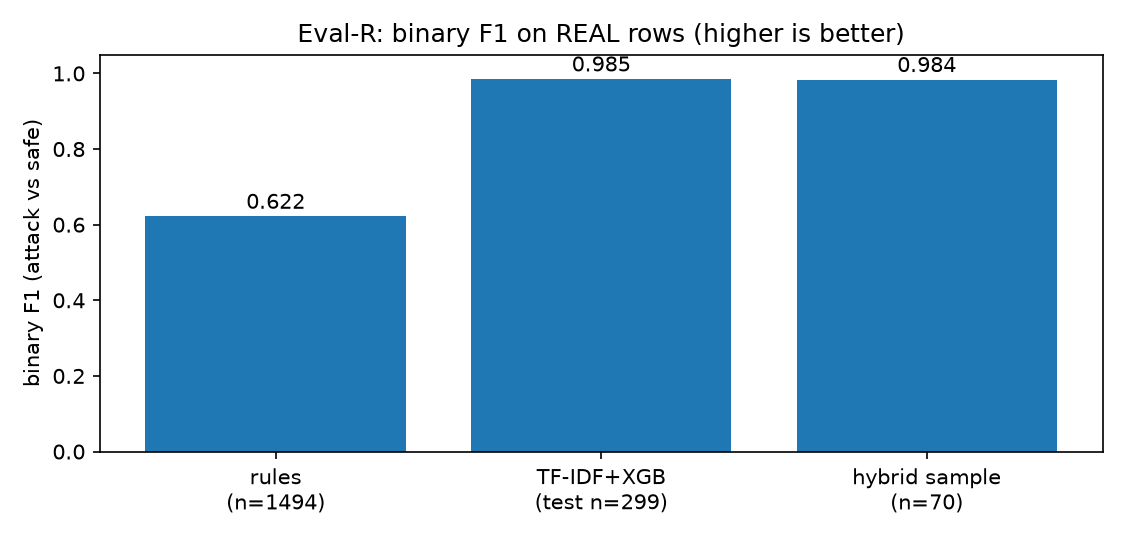
\includegraphics[width=0.9\linewidth]{figs/fig-evalR-F1.png}\caption{Eval-R binary F1 on REAL rows (N shown; same metric).}\end{figure}
\begin{figure}[h]\centering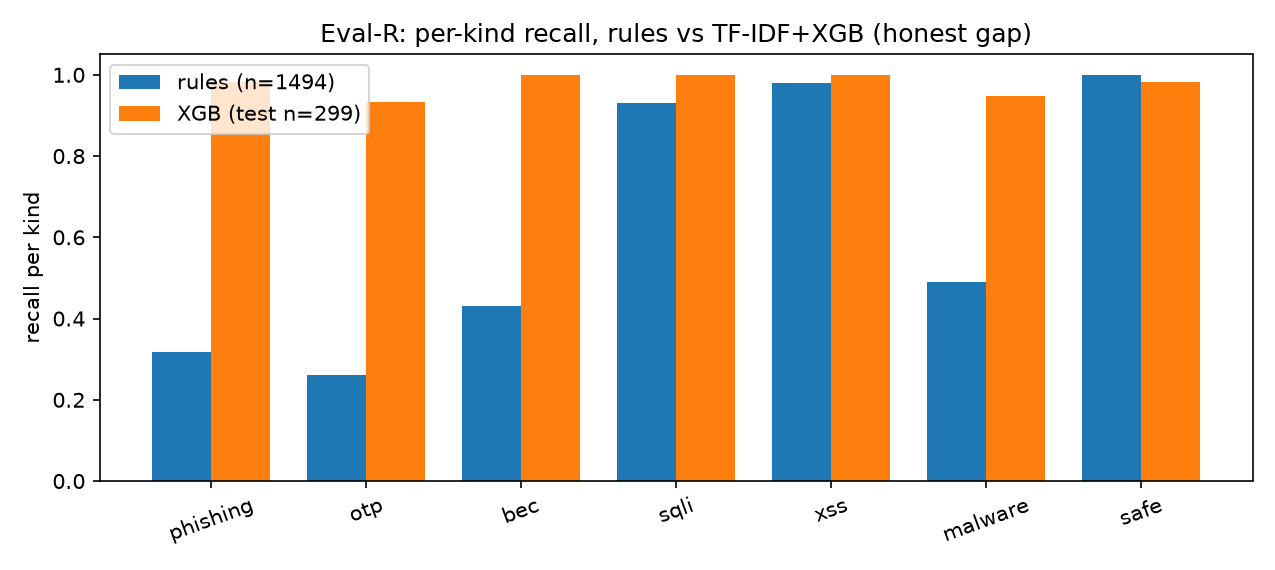
\includegraphics[width=0.9\linewidth]{figs/fig-perkind-recall.png}\caption{Eval-R per-kind recall, rules vs TF-IDF+XGB -- the honest gap (rules miss real phishing/otp/bec phrasing).}\end{figure}
\noindent\textit{Overleaf note:} upload the \texttt{docs/figs/} folder next to this \texttt{.tex} (files \texttt{fig-evalR-F1.png}, \texttt{fig-perkind-recall.png}).

\subsection{Ablation (briefed)}
Without the safety lock, the LLM marks some 0.6+ lures safe again \cite{Hasan25}. Without the medium stabilizer, mild lures flicker. Without kind-aware prompts, kind accuracy falls to rules-only BEC levels \cite{Ji25,CLASP25}. Lock on/off ablations on the Eval-R real set remain next work.

\subsection{Learning protocol -- humans pending (N=30)}
\texttt{EVAL\_B\_PACK} sets N=30: control reads static tips; treated staff ask three questions on /support and play voice + video; ten shared questions form pre/post tests; bar +15\% uplift at $p<0.05$; SUS usability \cite{EvalMethod24}. Follows in-field RCT and tutoring-gain precedents \cite{Vanzo25,Greco25,Pardos24,TutorCopilot24}. [To fill after the run.]

\subsection{Threats to validity}
v2 set overfits by construction; 70 cases are few; free-tier latency varies; Eval-B draws from one site; LLM path needs key + network; English prompts only. Eval-R limits: small classes stay small (sqli/xss 100, malware 94; test split 20/20/19), Fraud-R1 EN half only, SMS-ham style safe, hybrid measured on a 70-sample (cost), XGB on one 80/20 split (no k-fold yet).

\section{Discussion (briefed)}
\textit{What we learned:} the hard core is phishing vs otp vs bec -- rules under-fire BEC, the LLM at times over-reads prize wording as OTP pressure. The safety lock buys full recall on our 70 at almost no false-positive cost. Honest bounds stay: no packet sniff (REST + WS prototype) \cite{Rigaki24,Castro25}, Render cold start $\sim$30\,s \cite{Docker24}, slide video rather than avatar (paid API disclosed as limit), English only. Classical baselines: TF-IDF+XGBoost is now measured on Eval-R (F1 0.985, Sec~6); BERT/RF remain next \cite{Algo25,FinFraud25,BERT24}.

\section{Conclusion and Future Work}
We built and measured a seven-class closed loop with open tables and a runnable release: four agents, one hybrid model (no training), one orchestration (REST + WS), honest evals. Next: BERT/RF rerun on the Eval-R real set with k-fold, N=30 study \cite{Vanzo25,EvalMethod24}, multilingual voice, packet agent \cite{Rigaki24}, admin analytics, cascade cost control \cite{CLASP25} and red-team hardening \cite{SecEval225,AgentHarm25} pre-deploy. Code, builders and tables: \url{https://github.com/Koushiq-Sourav/finlearn_guard.git}.

\section*{Acknowledgments}
Supervision by Poly Rani Ghosh, Notre Dame University Bangladesh, whose demands for briefing, explicit agents/model/orchestration, 120+ references and a wider gap analysis shaped Rev.2. Thanks to open-source model, edge-tts and moviepy authors, and to the public benchmark teams cited above.

\begin{thebibliography}{120}
\bibitem{Heiding24} F. Heiding, B. Schneier, A. Vishwanath et al., Devising and Detecting Phishing Emails Using Large Language Models, IEEE Access, vol.~12, pp.~42131--42146, 2024. DOI:10.1109/ACCESS.2024.3375882. arXiv:2308.12287. \url{https://ieeexplore.ieee.org/document/10466545}
\bibitem{Koide24} T. Koide et al., ChatSpamDetector: Leveraging Large Language Models for Effective Phishing Email Detection, SecureComm 2024, arXiv:2402.18093. \url{https://arxiv.org/abs/2402.18093}
\bibitem{Desolda24} G. Desolda, F. Greco, L. Vigan\`o, APOLLO: A GPT-based tool to detect phishing emails and generate explanations that warn users, arXiv:2410.07997, 2024. \url{https://arxiv.org/abs/2410.07997}
\bibitem{Nair25} R. Nair, F. Abbasi, S. Pervez, PhishEmailLLM: A Meta Model Approach to Detect Phishing emails by leveraging LLMs and Machine Learning models, ACSW 2025, pp.~19--29. \url{https://dl.acm.org/doi/10.1145/3727166.3727169}
\bibitem{Algo25} S. Tarapiah et al., Evaluating the Effectiveness of LLMs Versus ML in Detecting Phishing Email Attempts, Algorithms, vol.~18, no.~10, p.~599, 2025. \url{https://www.mdpi.com/1999-4893/18/10/599}
\bibitem{SchoniCHI25} L. Sch\"oni et al., It's a Match -- Enhancing the Fit between Users and Phishing Training through Personalisation, CHI 2025. DOI:10.1145/3706598.3713845. \url{https://doi.org/10.1145/3706598.3713845}
\bibitem{SchoniEU24} L. Sch\"oni, V. Carles, M. Strohmeier, P. Mayer, V. Zimmermann, You Know What? -- Evaluation of a Personalised Phishing Training Based on Users' Knowledge and Skills, EuroUSEC 2024. DOI:10.1145/3688459.3688460. \url{https://doi.org/10.1145/3688459.3688460}
\bibitem{Sriganthan25} K. Sriganthan, F. H\"arer, An Adaptive Phishing Awareness Training Environment Based on LLMs and Interactive Learning, IEEE RTSI 2025, pp.~362--365. \url{https://2025.ieee-rtsi.org/}
\bibitem{TrainShield25} G. Pizzenti et al., TrainShield: Targeted Awareness for Cybersecurity Training, ACM Hypertext (HT) 2025. DOI:10.1145/3800935.3830870. arXiv:2608.02296. \url{https://doi.org/10.1145/3800935.3830870}
\bibitem{Greco25} F. Greco et al., Improving Phishing Resilience with AI-Generated Training: Evidence on Prompting, Personalization, and Duration, arXiv:2512.01893, 2025. N=480. \url{https://arxiv.org/abs/2512.01893}
\bibitem{DAMOCLES24} B. Breve et al.\ (eds.), Proc.\ First Int.\ Workshop on Detection And Mitigation Of Cyber attacks that exploit human vuLnerabilitiES (DAMOCLES 2024), AVI 2024, CEUR Vol.~3713. \url{https://ceur-ws.org/Vol-3713/}
\bibitem{Zhou25} L. Zhou, A. Aldkheel, Gamification-based Spear Phishing Awareness Training System: Four Novel Design Artifacts, AMCIS 2025. \url{https://authorconnect.aisnet.org/conferences/AMCIS2025/papers/1980}
\bibitem{SAGE26} Y. Chen et al., SAGE: An LLM-driven Self Reflective Agentic Framework for Fraud Detection, arXiv:2606.08146, 2026. \url{https://arxiv.org/abs/2606.08146}
\bibitem{RiskFirst26} Z. Chen et al., From Tasks to Teams: A Risk-First Evaluation Framework for Multi-Agent LLM Systems in Finance, Findings of ACL 2026, pp.~38819--38857. \url{https://aclanthology.org/2026.findings-acl.1934/}
\bibitem{AMLNet25} S. Huda et al., AMLNet: A Knowledge-Based Multi-Agent Framework to Generate and Detect Realistic Money Laundering Transactions, arXiv:2509.11595, 2025. \url{https://arxiv.org/abs/2509.11595}
\bibitem{AuditAgent25} S. Bai et al., AuditAgent: Expert-Guided Multi-Agent Reasoning for Cross-Document Fraudulent Evidence Discovery, arXiv:2510.00156, 2025. ICAIF 2025. \url{https://arxiv.org/abs/2510.00156}
\bibitem{AgenticCyber25} S. Roy, AgenticCyber: A GenAI-Powered Multi-Agent System for Multimodal Threat Detection and Adaptive Response, arXiv:2512.06396, 2025. \url{https://arxiv.org/abs/2512.06396}
\bibitem{MALCDF25} A. Bhardwaj et al., MALCDF: A Distributed Multi-Agent LLM Framework for Real-Time Cyber Defense, arXiv:2512.14846, 2025. \url{https://arxiv.org/abs/2512.14846}
\bibitem{CyLens25} X. Liu et al., CyLens: Towards Reinventing Cyber Threat Intelligence in the Paradigm of Agentic LLMs, arXiv:2502.20791, 2025. \url{https://arxiv.org/abs/2502.20791}
\bibitem{TradingAgents24} Y. Xiao et al., TradingAgents: Multi-Agents LLM Financial Trading Framework, arXiv:2412.20138, 2024. \url{https://arxiv.org/abs/2412.20138}
\bibitem{IJCISIM26} B. Biswas et al., A Framework for Agentic AI-Driven Financial Fraud Detection, Investigation, and Risk Mitigation in Real-Time Payment Ecosystems, IJCISIM, vol.~18, no.~3s, pp.~1029--1040, 2026. DOI:10.70917/ijcisim-2026-2434. \url{https://cspub-ijcisim.org/index.php/ijcisim/article/view/2434}
\bibitem{UserRAG26} A. H. Al Barwani et al., User-Centric Phishing Detection: A RAG and LLM-Based Approach, arXiv:2601.21261, 2026. \url{https://arxiv.org/abs/2601.21261}
\bibitem{MemoPhish26} X. Chen et al., MemoPhishAgent: Memory-Augmented Multi-Modal LLM Agent for Phishing URL Detection, ACL 2026 Industry, pp.~1182--1196. arXiv:2602.21394. \url{https://aclanthology.org/2026.acl-industry.84/}
\bibitem{Hasan25} N. Hasan et al., Phishing Email Detection Using LLMs (LLM-PEA), arXiv:2512.10104, 2025. \url{https://arxiv.org/abs/2512.10104}
\bibitem{Ji25} F. Ji, D. Kim, How Can We Effectively Use LLMs for Phishing Detection?, arXiv:2511.09606, 2025. \url{https://arxiv.org/abs/2511.09606}
\bibitem{CLASP25} F. Trad, A. Chehab, CLASP: Cost-Optimized LLM-based Agentic System for Phishing Detection, arXiv:2510.18585, 2025. \url{https://arxiv.org/abs/2510.18585}
\bibitem{HeidingIntent24} F. Heiding et al., Evaluating LLMs' Capability to Launch Fully Automated Spear Phishing Campaigns: Validated on Human Subjects, arXiv:2412.00586, 2024. \url{https://arxiv.org/abs/2412.00586}
\bibitem{FinFraud25} J. Chen et al., FinFraud-LLM: Exploring LLMs for Financial Fraud Detection, IEEE ICDMW Workshops 2025, pp.~3087--3091. DOI:10.1109/ICDMW69685.2025.00407. \url{https://ieeexplore.ieee.org/document/11416046}
\bibitem{FinFRE25} X. Tan et al., Understanding Structured Financial Data with LLMs: A Case Study on Fraud Detection (FinFRE-RAG), arXiv:2512.13040, 2025. \url{https://arxiv.org/abs/2512.13040}
\bibitem{SENSAI25} C. Nelson et al., SENSAI: LLMs as Applied Cybersecurity Tutors, SIGCSE TS 2025, vol.~1, pp.~833--839. DOI:10.1145/3641554.3701801. \url{https://doi.org/10.1145/3641554.3701801}
\bibitem{SYNAPSE26} G. Ferrara, A. Sami, SYNAPSE: A Multi-LLM Orchestrated AI Tutor for Secure Software Development Education, arXiv:2607.14601, 2026. ICSME 2026. \url{https://arxiv.org/abs/2607.14601}
\bibitem{Frazier26} M. Frazier, K. Damevski, Towards Personalizing Secure Programming Education with LLM-Injected Vulnerabilities, arXiv:2604.13955, 2026. N=71. \url{https://arxiv.org/abs/2604.13955}
\bibitem{CurricuLLM26} A. Nijdam et al., CurricuLLM: Designing Personalized and Workforce-Aligned Cybersecurity Curricula Using Fine-Tuned LLMs, arXiv:2601.04940, 2026. \url{https://arxiv.org/abs/2601.04940}
\bibitem{CyberMentor25} T. Wang et al., CyberMentor: AI Powered Learning Tool Platform for Diverse Cyber Students, arXiv:2501.09709, 2025. \url{https://arxiv.org/abs/2501.09709}
\bibitem{CyberQ24} G. Agrawal et al., CyberQ: Generating Questions and Answers for Cybersecurity Education Using Knowledge Graph-Augmented LLMs, AAAI 2024, vol.~38, no.~21, pp.~23164--23172. \url{https://doi.org/10.1609/aaai.v38i21.30362}
\bibitem{FraudR125} S. Yang et al., Fraud-R1: A Multi-Round Benchmark for Assessing Robustness of LLMs Against Augmented Fraud and Phishing, arXiv:2502.12904, 2025. ACL Findings 2025. \url{https://arxiv.org/abs/2502.12904}
\bibitem{FraudBench25} Q. Ren et al., When AI Agents Collude Online: Financial Fraud Risks by Collaborative LLM Agents (MultiAgentFraudBench), arXiv:2511.06448, 2025. \url{https://arxiv.org/abs/2511.06448}
\bibitem{FinSafety26} FinSafetyBench: Evaluating LLM Safety in Real-World Financial Scenarios, arXiv:2605.00706, 2026. \url{https://arxiv.org/abs/2605.00706}
\bibitem{XFin25} Z. Zhang et al., XFinBench: Benchmarking LLMs in Complex Financial Problem Solving and Reasoning, arXiv:2508.15861, 2025. ACL 2025. \url{https://arxiv.org/abs/2508.15861}
\bibitem{FinBen24} Q. Xie et al., FinBen: A Holistic Financial Benchmark for LLMs, NeurIPS 2024 Datasets and Benchmarks. \url{https://proceedings.neurips.cc/paper_files/paper/2024/file/adb1d9fa8be4576d28703b396b82ba1b-Paper-Datasets_and_Benchmarks_Track.pdf}
\bibitem{FinAgentBench25} A. Bigeard et al., Finance Agent Benchmark: Benchmarking LLMs on Real-world Financial Research Tasks, arXiv:2508.00828, 2025. 537 tasks. \url{https://arxiv.org/abs/2508.00828}
\bibitem{Investor25} InvestorBench: Benchmarking LLMs for Financial Decision-Making, ACL 2025, long paper, pp.~2509--2525. \url{https://aclanthology.org/2025.acl-long.126.pdf}
\bibitem{FangHack24} R. Fang et al., LLM Agents can Autonomously Hack Websites, arXiv:2402.06664, 2024. \url{https://arxiv.org/abs/2402.06664}
\bibitem{FangExploit24} R. Fang et al., LLM Agents can Autonomously Exploit One-day Vulnerabilities, arXiv:2404.08144, 2024. \url{https://arxiv.org/abs/2404.08144}
\bibitem{PentestGPT24} G. Deng et al., PentestGPT: Evaluating and Harnessing LLMs for Automated Penetration Testing, Proc.\ 33rd USENIX Security 2024, pp.~847--864. arXiv:2308.06782. \url{https://www.usenix.org/conference/usenixsecurity24/presentation/deng}
\bibitem{Rigaki24} M. Rigaki et al., Hackphyr: A Local Fine-Tuned LLM Agent for Network Security Environments, arXiv:2409.11276, 2024. \url{https://arxiv.org/abs/2409.11276}
\bibitem{IDSAgent24} Y. Li, Z. Xiang, N. Bastian, D. Song, B. Li, IDS-Agent: An LLM Agent for Explainable Intrusion Detection in IoT Networks, NeurIPS 2024 Workshop on Open-World Agents (OWA). F1 0.97/0.75, zero-day recall 0.61. \url{https://openreview.net/forum?id=iiK0pRyLkw}
\bibitem{Houssel24} P. R. B. Houssel, P. Singh, S. Layeghy, M. Portmann, Towards Explainable Network Intrusion Detection using Large Language Models, arXiv:2408.04342, 2024. IEEE/ACM BDCAT 2024, pp.~67--72. \url{https://arxiv.org/abs/2408.04342}
\bibitem{Tellache25} A. Tellache, A. A. Korba, A. Mokhtari et al., Advancing Autonomous Incident Response: Leveraging LLMs and Cyber Threat Intelligence, arXiv:2508.10677, 2025. RAG + CTI response generation. \url{https://arxiv.org/abs/2508.10677}
\bibitem{Castro25} S. R. Castro et al., Large Language Models are Autonomous Cyber Defenders, IEEE CAI 2025, pp.~1125--1132. CAGE-4 multi-agent LLM+RL. arXiv:2505.04843. \url{https://arxiv.org/abs/2505.04843}
\bibitem{Saju26} M. H. Saju, A. Azim, Toward Autonomous SOC Operations: End-to-End LLM Framework for Threat Detection, Query Generation, and Resolution, PMLR, vol.~318, pp.~422--433, 2026. Canadian AI 2026. \url{https://proceedings.mlr.press/v318/saju26a.html}
\bibitem{Honeypot24} Reworr, D. Volkov, LLM Agent Honeypot: Monitoring AI Hacking Agents in the Wild, arXiv:2410.13919, 2024. 8M attempts, 8 AI agents. \url{https://arxiv.org/abs/2410.13919}
\bibitem{SAGA25} G. Syros et al., SAGA: A Security Architecture for Governing AI Agentic Systems, arXiv:2504.21034, 2025. NDSS 2026. \url{https://arxiv.org/abs/2504.21034}
\bibitem{Aegis25} Z. Cai et al., AegisLLM: Scaling Agentic Systems for Self-Reflective Defense in LLM Security, arXiv:2504.20965, 2025. ICLR 2025 Workshop. \url{https://arxiv.org/abs/2504.20965}
\bibitem{AIR26} Z. Xiao et al., AIR: Improving Agent Safety through Incident Response, arXiv:2602.11749, 2026. ICML 2026. \url{https://arxiv.org/abs/2602.11749}
\bibitem{Park24} T. Park, Enhancing Anomaly Detection in Financial Markets with an LLM-based Multi-Agent Framework, arXiv:2403.19735, 2024. \url{https://arxiv.org/abs/2403.19735}
\bibitem{FinAgent24} W. Zhang et al., FinAgent: A Multimodal Foundation Agent for Financial Trading, KDD 2024, pp.~4314--4325. arXiv:2402.18485. \url{https://doi.org/10.1145/3637528.3671801}
\bibitem{FinCon24} Y. Yu et al., FinCon: A Synthesized LLM Multi-Agent System with Conceptual Verbal Reinforcement for Financial Decision Making, NeurIPS 2024, pp.~137010--137045. arXiv:2407.06567. \url{https://arxiv.org/abs/2407.06567}
\bibitem{HedgeAgents25} X. Li et al., HedgeAgents: A Balanced-aware Multi-agent Financial Trading System, WWW Companion 2025, pp.~296--305. arXiv:2502.13165. \url{https://arxiv.org/abs/2502.13165}
\bibitem{FinRobot24} H. Yang et al., FinRobot: An Open-Source AI Agent Platform for Financial Applications using LLMs, arXiv:2405.14767, 2024. \url{https://arxiv.org/abs/2405.14767}
\bibitem{Collude25} Q. Ren et al., When AI Agents Collude Online: Financial Fraud Risks by Collaborative LLM Agents, ICLR 2026. arXiv:2507.14660, 2025. \url{https://arxiv.org/abs/2507.14660}
\bibitem{Qu25} B. Qu et al., LLM-Enhanced Self-Evolving Reinforcement Learning for Multi-Step E-Commerce Payment Fraud Risk Detection, ACL Industry 2025, pp.~92--103. \url{https://aclanthology.org/2025.acl-industry.9/}
\bibitem{AutoGen24} V. Dibia et al., AutoGen Studio: A No-Code Developer Tool for Building and Debugging Multi-Agent Systems, arXiv:2408.15247, 2024. \url{https://arxiv.org/abs/2408.15247}
\bibitem{Lee25} C. Lee, Enhancing Phishing Email Identification with Large Language Models, arXiv:2502.04759, 2025. \url{https://arxiv.org/abs/2502.04759}
\bibitem{Kuikel25} S. Kuikel et al., Evaluating LLMs for Phishing Detection, Self-Consistency, Faithfulness, and Explainability, arXiv:2506.13746, 2025. \url{https://arxiv.org/abs/2506.13746}
\bibitem{MultiGuard25} Y. Xue et al., MultiPhishGuard: An Explainable and Adaptive Multi-Agent LLM System for Phishing Email Detection, arXiv:2505.23803, 2025. \url{https://arxiv.org/abs/2505.23803}
\bibitem{PhishDebate25} W. Li et al., PhishDebate: An LLM-Based Multi-Agent Framework for Phishing Website Detection, arXiv:2506.15656, 2025. IEEE BigData 2025. \url{https://arxiv.org/abs/2506.15656}
\bibitem{NextGenPhish24} K. Afane et al., Next-Generation Phishing: How LLM Agents Empower Cyber Attackers, arXiv:2411.13874, 2024. \url{https://arxiv.org/abs/2411.13874}
\bibitem{MMPhish24} J. Lee et al., Multimodal LLMs for Phishing Webpage Detection and Identification, arXiv:2408.05941, 2024. \url{https://arxiv.org/abs/2408.05941}
\bibitem{KnowPhish24} Y. Li et al., KnowPhish: LLMs Meet Multimodal Knowledge Graphs for Reference-Based Phishing Detection, Proc.\ 33rd USENIX Security 2024, pp.~793--810. \url{https://www.usenix.org/conference/usenixsecurity24/presentation/li-yuexin}
\bibitem{PhishAgent25} Y. Cao et al., PhishAgent: A Robust Multimodal Agent for Phishing Webpage Detection, AAAI 2025, vol.~39, no.~27, pp.~27869--27877. arXiv:2408.10738. \url{https://ojs.aaai.org/index.php/AAAI/article/view/35003}
\bibitem{PhishOracle24} R. Kulkarni et al., From ML to LLM: Evaluating Robustness of Phishing Webpage Detection Models against Adversarial Attacks (PhishOracle), arXiv:2407.20361, 2024. \url{https://arxiv.org/abs/2407.20361}
\bibitem{PhishLang24} S. Roy, S. Nilizadeh, PhishLang: A Real-Time, Fully Client-Side Phishing Detection Framework Using MobileBERT, arXiv:2408.05667, 2024. \url{https://arxiv.org/abs/2408.05667}
\bibitem{OneShotURL24} F. Rashid et al., LLMs are One-Shot URL Classifiers and Explainers, arXiv:2409.14306, 2024. \url{https://arxiv.org/abs/2409.14306}
\bibitem{KorSmish24} J. Lee, D. Han, KorSmishing Explainer: Korean-centric LLM-based Framework for Smishing Detection and Explanation, EMNLP 2024 Industry, pp.~642--656. \url{https://aclanthology.org/2024.emnlp-industry.47/}
\bibitem{SmishX25} Y. Wang et al., Can You Walk Me Through It? Explainable SMS-Phishing Detection Using LLM-Based Agents (SmishX), SOUPS 2025, pp.~37--56. N=175. \url{https://www.usenix.org/conference/soups2025/presentation/wang}
\bibitem{SpaLLM25} S. Salman et al., SpaLLM-Guard: Pairing SMS Spam Detection Using Open-source and Commercial LLMs, arXiv:2501.04985, 2025. \url{https://arxiv.org/abs/2501.04985}
\bibitem{COPS24} Harichandana et al., COPS: A Compact On-device Pipeline for real-time Smishing detection, IEEE CCNC 2024, pp.~172--179. arXiv:2402.04173. \url{https://arxiv.org/abs/2402.04173}
\bibitem{SmishCheck25} Schwarz et al., Zero-training fraud detection in a large messaging platform (Smish-Checker: threefold campaign + LLM + propagation), WACV 2025 Workshop AI4MFDD. \url{https://openaccess.thecvf.com/content/WACV2025W/AI4MFDD/papers/Schwarz_Zero-training_fraud_detection_in_a_large_messaging_platform_WACVW_2025_paper.pdf}
\bibitem{Persuade24} Shim et al., Data augmentation for smishing detection: A theory-based prompt engineering approach, WWW Companion 2024, pp.~1327--1328. arXiv:2411.02403. \url{https://arxiv.org/abs/2411.02403}
\bibitem{MozSmish25} Ali et al., MOZ-Smishing: Benchmark Dataset for Detecting Mobile Money Frauds, AfricaNLP 2025, pp.~158--166. \url{https://aclanthology.org/2025.africanlp-1.23}
\bibitem{BECReview25} A. Almutairi et al., Business email compromise: a systematic review of understanding, detection, and challenges, Computers \& Security, vol.~158, p.~104630, 2025. DOI:10.1016/j.cose.2025.104630. \url{https://doi.org/10.1016/j.cose.2025.104630}
\bibitem{StruQ24} S. Chen et al., StruQ: Defending Against Prompt Injection with Structured Queries, arXiv:2402.06363, 2024. Proc.\ USENIX Security 2025, pp.~2383--2400. \url{https://www.usenix.org/conference/usenixsecurity25/presentation/chen-sizhe}
\bibitem{Hierarchy24} J. Wallace et al., Instruction Hierarchy: Teaching LLMs to Prioritize Privileged Instructions, arXiv:2404.13208, 2024. \url{https://arxiv.org/abs/2404.13208}
\bibitem{PromptVsTune24} F. Trad, A. Chehab, Prompt Engineering or Fine-Tuning? A Case Study on Phishing Detection with LLMs, Machine Learning and Knowledge Extraction, vol.~6, no.~1, pp.~367--384, 2024. \url{https://www.mdpi.com/2504-4990/6/1/18}
\bibitem{Pardos24} Z. A. Pardos, S. Bhandari, ChatGPT-generated help produces learning gains equivalent to human tutor-authored help, PLoS ONE, vol.~19, no.~5, e0304013, 2024. N=274. \url{https://doi.org/10.1371/journal.pone.0304013}
\bibitem{TutorCopilot24} R. E. Wang et al., Tutor CoPilot: A Human-AI Approach for Scaling Real-Time Expertise, arXiv:2410.03017, 2024. N=1800. \url{https://arxiv.org/abs/2410.03017}
\bibitem{Kestin25} G. Kestin et al., AI tutoring outperforms in-class active learning: an RCT introducing a novel research-based design, Scientific Reports, vol.~15, p.~17458, 2025. N=194. \url{https://www.nature.com/articles/s41598-025-97652-6}
\bibitem{Khanmigo25} P. Oreopoulos, N. Low, One Click Away: AI Tutoring with Khanmigo in a Two-Year School Experiment, NBER Working Paper 35620, 2026. Trials 2024--2026. \url{https://www.nber.org/papers/w35620}
\bibitem{Vanzo25} A. Vanzo et al., GPT-4 as a Homework Tutor Can Improve Student Engagement and Learning Outcomes, Proc.\ ACL 2025, long paper, pp.~31119--31136. \url{https://aclanthology.org/2025.acl-long.1502/}
\bibitem{Blasco24} M. Blasco, C. Charisi, AI Chatbots in K-12 Education: Socratic vs Non-Socratic and Role of Step-by-Step Reasoning, SSRN 5040921, Dec 2024. N=122. \url{https://papers.ssrn.com/sol3/papers.cfm?abstract_id=5040921}
\bibitem{Lain24} D. Lain et al., Phishing in Organizations: Embedding Training and Awareness, Proc.\ ACM CCS 2024. Timely nudges beat long content.
\bibitem{GrecoCEUR24} G. Desolda, F. Greco, L. Vigan\`o, Supporting Design of Phishing Education, Training and Awareness interventions: LLM-based approach, Proc.\ CSE4IA 2024, CEUR Vol.~3700, paper 8. \url{https://ceur-ws.org/Vol-3700/paper8.pdf}
\bibitem{FinQA24} F. Fatemi, H. Hu, Enhancing financial question answering with a multi-agent reflection framework, ICAIF 2024, pp.~530--537.
\bibitem{Cybench25} Z. Zhang et al., Cybench: Framework for Evaluating Cybersecurity Capabilities and Risks of Language Models, ICLR 2025. arXiv:2408.08926. \url{https://arxiv.org/abs/2408.08926}
\bibitem{SecEval225} M. Bhatt et al., CyberSecEval 2: Wide-Ranging Cybersecurity Evaluation Suite, arXiv:2404.13161, 2024. \url{https://arxiv.org/abs/2404.13161}
\bibitem{SecEval325} L. Wan et al., CYBERSECEVAL 3: Advancing Evaluation of Cybersecurity Risks and Capabilities, arXiv:2408.01605, 2024. \url{https://arxiv.org/abs/2408.01605}
\bibitem{AgentHarm25} M. Andriushchenko et al., AgentHarm: Benchmark for Measuring Harmfulness of LLM Agents, ICLR 2025. arXiv:2410.09024. \url{https://arxiv.org/abs/2410.09024}
\bibitem{HarmBench24} M. Mazeika et al., HarmBench: Standardized Evaluation Framework for Automated Red Teaming, ICML 2024. arXiv:2402.04249. \url{https://arxiv.org/abs/2402.04249}
\bibitem{SWEbench24} C. Jimenez et al., SWE-bench: Can Language Models Resolve Real-World GitHub Issues?, ICLR 2024. \url{https://openreview.net/forum?id=VTF8yNQM66}
\bibitem{AgentBench24} X. Liu et al., AgentBench: Evaluating LLMs as Agents, ICLR 2024. arXiv:2308.03688. \url{https://arxiv.org/abs/2308.03688}
\bibitem{SWEagent24} J. Yang et al., SWE-agent: Agent-Computer Interfaces Enable Automated Software Engineering, NeurIPS 2024. arXiv:2405.15793. \url{https://arxiv.org/abs/2405.15793}
\bibitem{FastAPI24} S. Ram\'irez, FastAPI documentation, 2024. Uvicorn and Jinja2 and WebSocket support. \url{https://fastapi.tiangolo.com/}
\bibitem{Mongo24} MongoDB, MongoDB Atlas documentation, 2024. \url{https://www.mongodb.com/docs/atlas/}
\bibitem{EdgeTTS24} edge-tts: Text-to-speech with Microsoft Edge Read Aloud, 2024. \url{https://github.com/rany2/edge-tts}
\bibitem{Moviepy24} moviepy and imageio-ffmpeg documentation, 2024. \url{https://zulko.github.io/moviepy/}
\bibitem{HTTPX24} httpx: A next-generation HTTP client for Python, 2024. \url{https://www.python-httpx.org/}
\bibitem{Pytest24} pytest documentation, 2024. \url{https://docs.pytest.org/}
\bibitem{Docker24} Docker and Render deployment documentation, 2024. \url{https://docs.docker.com/} \url{https://render.com/docs}
\bibitem{OWASP24} OWASP Foundation, OWASP Top 10:2021, 2024 update. \url{https://owasp.org/Top10/}
\bibitem{NIST24} NIST, Computer Security Incident Handling Guide, SP 800-61 Rev.~3, 2024. Threat classes grounding. \url{https://csrc.nist.gov/pubs/sp/800/61/r3/final}
\bibitem{PyStd24} Python Software Foundation, Python 3.13 standard library documentation (subprocess, socket, netstat/ipconfig via OS), 2024. \url{https://docs.python.org/3.13/library/}
\bibitem{BERT24} J. Devlin et al., BERT: Pre-training of Deep Bidirectional Transformers for Language Understanding, NAACL 2019; Random Forest and XGBoost baselines: scikit-learn and Chen et al.\ 2016. \url{https://arxiv.org/abs/1810.04805}
\bibitem{EvalMethod24} J. Brooke, SUS: A quick and dirty usability scale, 1996; Student, The probable error of a mean, Biometrika, vol.~6, no.~1, pp.~1--25, 1908. For paired t-test and SUS in Eval-B protocol. \url{https://www.measuringu.com/sus/}
\bibitem{ZhangSME25} J. Zhang et al., Benchmarking and Evaluating LLMs in Phishing Detection for Small and Midsize Enterprises: A Comprehensive Analysis, IEEE Access, vol.~13, pp.~28335--28352, 2025. DOI:10.1109/ACCESS.2025.3534567. \url{https://ieeexplore.ieee.org/document/10878987}
\bibitem{OWASPASVS24} OWASP Foundation, Application Security Verification Standard (ASVS) 4.0: input validation and output encoding for sqli/xss, 2024. \url{https://owasp.org/www-project-application-security-verification-standard/}
\bibitem{NISTCSF24} NIST, Cybersecurity Framework (CSF) 2.0: Govern, Identify, Protect, Detect, Respond, Recover, 2024. \url{https://www.nist.gov/cyberframework}
\bibitem{RFC6455} I. Fette, A. Melnikov, The WebSocket Protocol, RFC 6455, IETF, 2011. Live push channel standard. \url{https://www.rfc-editor.org/rfc/rfc6455}
\bibitem{Jinja24} Pallets, Jinja2 template documentation, 2024. Server-side rendering. \url{https://jinja.palletsprojects.com/}
\bibitem{Codebook24} Saka et al., Phishing Codebook: Structured Framework for Characterization of Phishing Emails, arXiv:2408.08967, 2024. \url{https://arxiv.org/abs/2408.08967}
\end{thebibliography}
\end{document}
